
\documentclass[twocolumn,showpacs,%
  nofootinbib,aps,superscriptaddress,%
  eqsecnum,prd,notitlepage,showkeys,10pt]{revtex4-1}

\usepackage{amssymb}
\usepackage{amsmath}
\usepackage{graphicx}
\usepackage{dcolumn}
\usepackage{hyperref}
\usepackage{helvet}
\usepackage{color}
\renewcommand{\familydefault}{\sfdefault}
\newcommand*{\TitleFont}{%
      \usefont{\encodingdefault}{\rmdefault}{b}{n}%
      \fontsize{16}{20}%
      \selectfont}

\begin{document}

\title{\TitleFont Calorinator - an interactive floor game to perform fitness exercises}
\author{Carl Ambroselli, Julius Treike, Marc-Philipp Bismar, Marvin Bornstein}
\affiliation{Hasso-Plattner-Institute\\Potsdam}

% \begin{abstract}
% Your abstract.
% \end{abstract}

\maketitle

\section{Abstract}

We introduce a jump 'n' run game for interactive floors to maintain body fitness. Players control themselves directly by stepping, jumping or laying on the   floor.

In a forrest, users jump over fallen trees or cross an ocean by holding themselves on ice floes. Repairing a bridge in shortage of time or similar complex    tasks pack fitness exercises in an exciting adventure. This motivates users to do regular physical activity.

\section{Introduction}

The modern society is changing the way we create our day to day life. More and more tasks are getting automated and are done by machines. This causes people to increase their time off from physical activities.
To reinsure people don’t loose their level of fitness they are signing up for fitness studios and try to force themselves to do sports more frequently.  This restrain to visit resolves in a lack of motivation. Only one third of gym members are trains once or more per week.
But by using bodyweight exercises people are able to perform a workout as effective as in the gym without the actual additional problems a fitness studio causes like e.g. the time you need for the way or the public display of their physical abilities.

\section{Walkthrough}

In this scenario the student Andy trains his body by running in place, jumping a lot, staying in push-ups position and alternating running and touching the floor.

\textcolor{white}{
Text Text Text Text Text Text Text Text Text Text Text Text Text Text Text Text Text Text Text Text Text Text Text Text Text Text Text Text Text Text Text Text Text Text Text Text Text Text Text Text Text Text Text Text Text Text
Text Text Text Text Text Text Text Text Text Text Text Text Text Text Text Text Text Text Text Text Text Text Text Text Text Text Text Text Text Text Text Text Text Text Text Text Text Text Text Text Text Text Text Text Text Text
Text Text Text Text Text Text Text Text Text Text Text Text Text Text Text Text Text Text Text Text Text Text Text Text Text Text Text Text Text Text Text Text Text Text Text Text Text Text Text Text Text Text Text Text Text Text
Text Text Text Text Text Text Text Text Text Text Text Text Text Text Text Text Text Text Text Text Text Text Text Text Text Text Text Text Text Text Text Text Text Text Text Text Text Text Text Text Text Text Text Text Text Text
}

\begin{figure}[!htb]
\minipage{0.5\textwidth}
  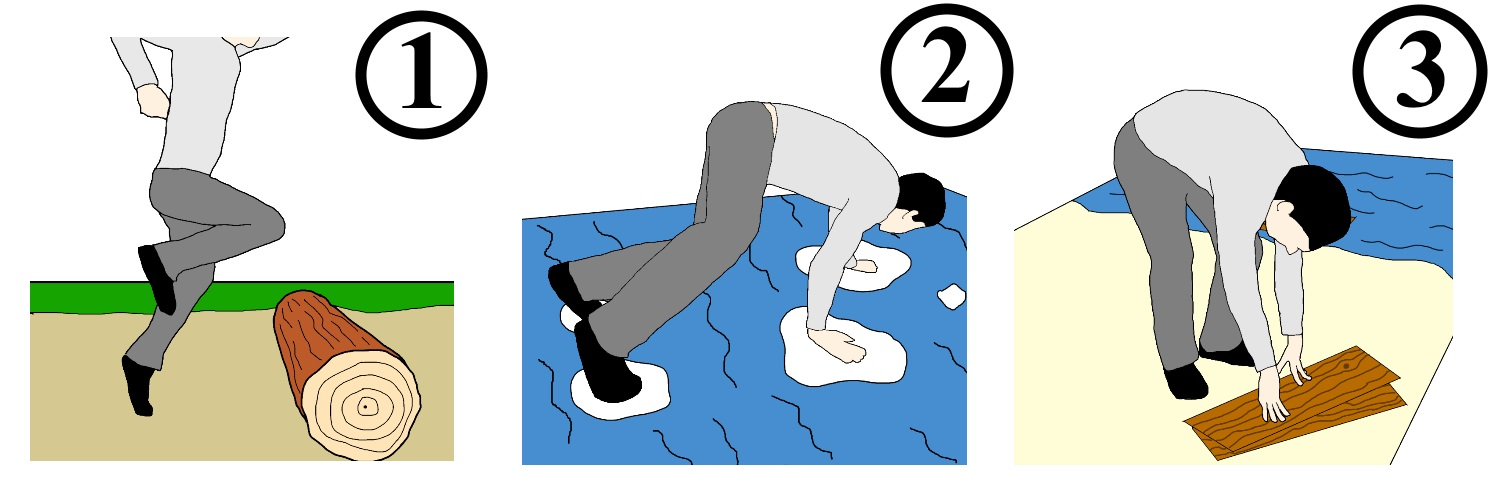
\includegraphics[width=\linewidth]{graphics/Image(11).jpg}
\endminipage\hfill
  \caption{Task Overview. (1) Andy runs in place and jumps over trees. (2) Water appeared  with some ice floes on it and Andy has to stay on these, but they melt. (3) Andy has to build a bridge to cross the water.}\label{fig:awesome_image3}
\end{figure}

The conrete beginning of the game (Figure 3 (1)) includes more thoughts. We focus on it in detail.

\begin{figure}[!htb]
\minipage{0.5\textwidth}
  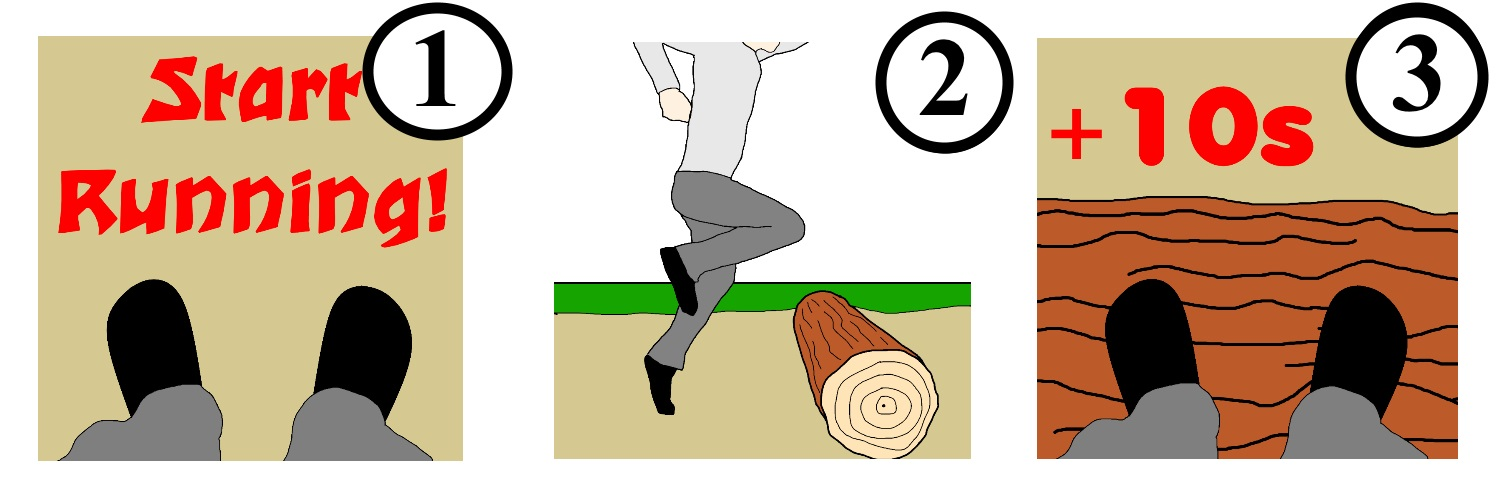
\includegraphics[width=\linewidth]{graphics/Image(12).jpg}
\endminipage\hfill
  \caption{(1) Andy is entering the floor and immediatly instructed to start running. The floor will begin to move under his feet. (2) When trees appear on the way, Andy has to jump over them. (3) When Andy unintentionally lands on a tree, he is punished with extra time (time is counting forwarsds and stopped, when one run is finished).}\label{fig:awesome_image3}
\end{figure}

\begin{figure}[!htb]
\minipage{0.5\textwidth}
  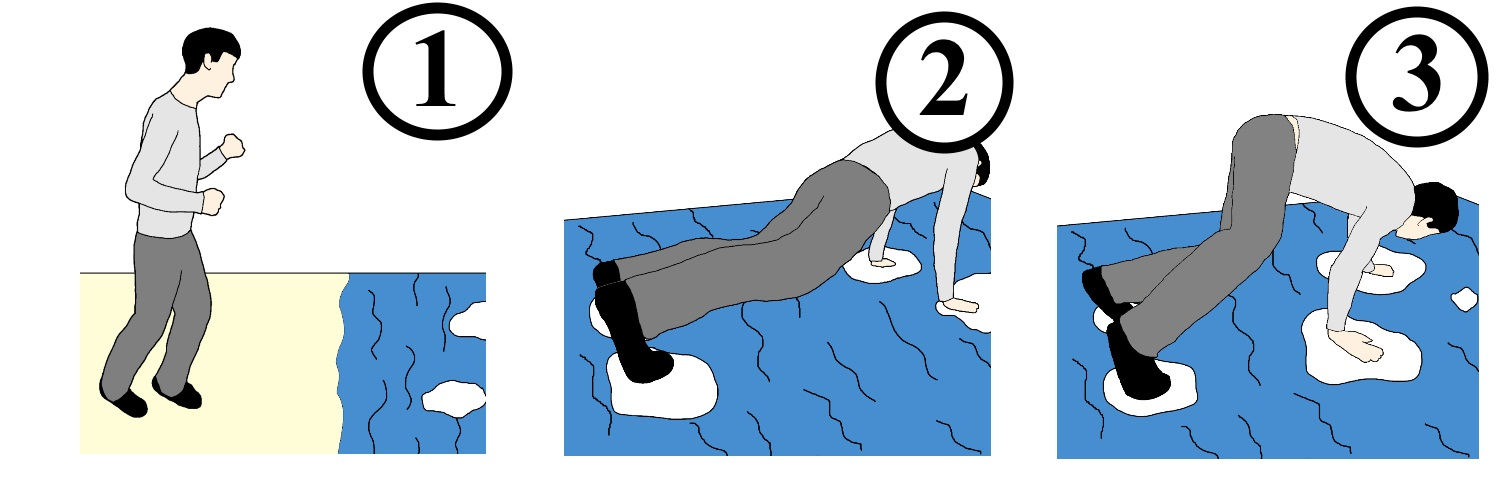
\includegraphics[width=\linewidth]{graphics/Image(13).jpg}
\endminipage\hfill
  \caption{(1) Andy runs over a beach and approaches water with ice floes on it. He is instructed to jump on them. (2) After jumping on the icefloes, he put his hand onto the other ice floes. (3) When an ice floe melts, others appear, Andy has to put the hand on.}\label{fig:awesome_image3}
\end{figure}


After a the ice floe game, the run proceeds as already shown in figure 3.

\begin{figure}[!htb]
\minipage{0.5\textwidth}
  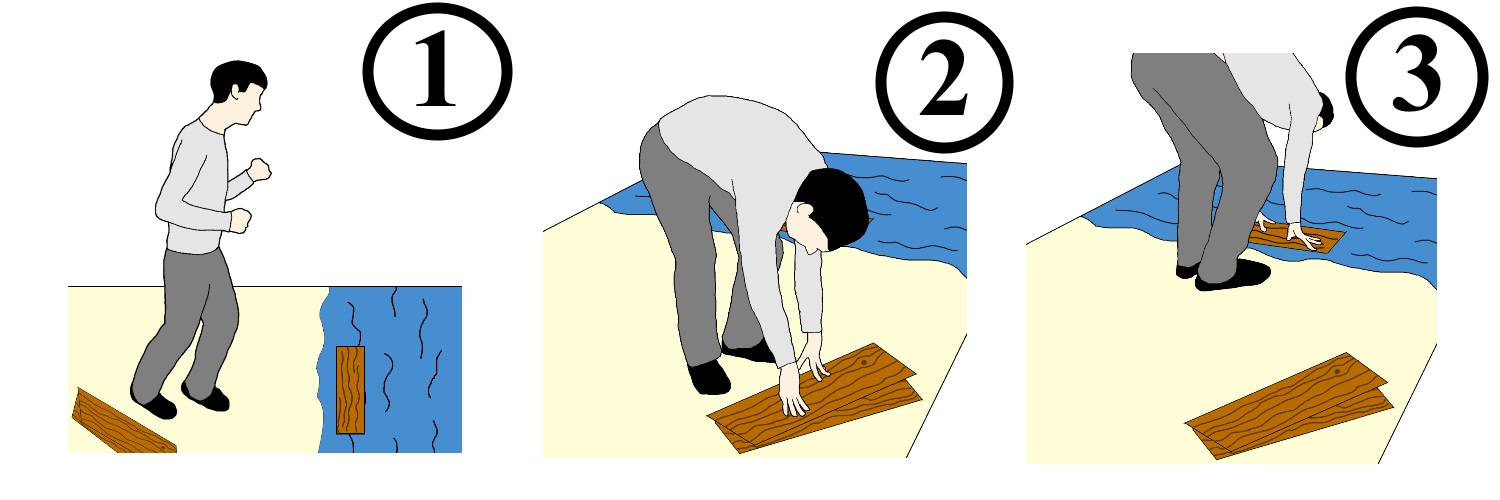
\includegraphics[width=\linewidth]{graphics/Image(14).jpg}
\endminipage\hfill
  \caption{(1) Andy runs over a beach with wood planks and is instructed to build a bridge to cross the water. (2) Andy touches the floor with his hands on the woodplanks to collect one. (3) He touches the water to build a part of a bridge. (4) Andy did alternating (2) and (3), finished the bridge and proceeds his run.}\label{fig:awesome_image3}
\end{figure}

% Commands to include a figure:
%\begin{figure}
%\includegraphics[width=\textwidth]{your-figure's-file-name}
%\caption{\label{fig:your-figure}Caption goes here.}
%\end{figure}

\section{Design}

\subsection{Instantly start game}

We had several iterations when to start a workout. Ideas like special locations like fitness mat turned out to be bad since the user did not understand them  when testing with a paper prototype. In the final version we chose to start the game as soon as someone starts running on the floor to provide the simplest   solution as possible.

During heuristic evaluation we identified that there must be a short message telling the user that he should start running, from that point on he understood  how to start a workout and make progress.

\subsection{Dictate Exercises}

In the early designs, we decided to let users choose the exercise they want to do and guide them in their performance. Possible tasks were to train you legs  for n seconds or build up strength performing n short, but hard exercises.

Within tast analysis, we noticed that this violates the need for a short workout, because much time is spent in the menu on selecting workouts. In our paper  prototype study two out of our 3 participants did not even know what the exercises are about or what kind of training they are. Users rather wanted to be     guided and told what would be best to do.

In the further process we reduced the options down to only 'warmup' or 'workout'. In the final design, we have a complete world with several workouts packed  in mini games.

\section{Conclusions}
When designing applications for interactive floors, user studies and exploration with prototypes becomes extremely imporant since there are no general patterns and the problem domain is yet unexplored. During the process our evaluation of the user's needs changed radically. When asking users what they wanted they looked at existing solutions and tried to map them to the floor. If we followed those, we would have ended up with a fitness mat and a video player. But this is already the solution for people, who want to do fitness without any sport equipment. We collected important aspects from users like the   need for motivation and limited free time and mapped them to possible exersices on the floor. Finally we came to the conclusion, that games are the most interactive solution that motivate users with fun when they work out. The ability to challenge your high score pushes your goals and shows you your progress.
Since developing an interactive protoype for a floor requires a major amount of work, paper prototyping turned out to be a powerful tool to find design flaws in your prototypes as users were able to imagine the system.
In addition, even when users want to use an application to do fitness activity, they look for the simplest solution to solve a game. Therefore you need to design fitness games that force users to do certain activity with the desired path instead of giving them the freedom how they want to solve a certain task.

\end{document}
